\section{Sensore} \label{sec:sensore}
Importante premessa prima di continuare con questa sezione: siccome oggi la fotografia si fa più in digitale che su pellicola, questo capitolo (come d'altronde il resto del manuale) è dedicato alla fotografia digitale, e quindi si parlerà si sensori; è bene però sapere che tutto ciò che verrà detto (meno i dettagli più specifici dell'elettronica dietro i sensori) vale anche per le pellicole.


\subsection{Full frame e APS-C} \label{subsec:sensorifullaps}
Nei primi anni della fotografia si usavano pellicole molto grandi e di varie dimensioni, poi negli anni è diventato molto diffuso a livello commerciale il formato \textbf{35mm}, anche detto \textbf{135} o \textbf{full frame}.
Le dimensioni di un sensore full frame sono $36mm \times 24mm$, per un rapporto base:altezza di 3:2.

Non a caso un formato classico per la stampa delle foto è $10 \times 15$ (in questo caso centimetri), che ha proprio lo stesso rapporto del sensore, ovvero 3:2.

Con l'avvento del digitale si sono diffusi sensori di dimensioni più contenute, mirati a fare fotocamere più economiche, che possono montare obiettivi più piccoli, leggeri e meno costosi delle controparti full-frame.
Lo scotto da pagare per un sensore più piccolo è una minore risoluzione, peggiore tollerabilità a ISO alti (i.e. le immagini hanno più rumore) e in generale una qualità di immagine inferiore; questo ovviamente va sempre rapportato da modello a modello: un sensore piccolo fatto oggi è comunque migliore di un sensore full frame dei primi anni 2000.

Quanto sono grandi questi sensori più piccoli? Non c'è un solo formato standard, ed ogni azienda usa un tipo di sensore.\newline
Canon usa sensori \textbf{APS-C}, \textbf{Advanced Photo System - Classic}. Anche Nikon usa sensori chiamati APS-C, ma quelli Nikon sono poco più grandi degli APS-C della Canon. Altro sensore molto importante è il \textbf{Micro 4/3}, di proprietà di Olympus e Panasonic.

\begin{multicols}{3}
    \begin{figure}
        %\centering
        
\includegraphics[width=0.2\textwidth]{FullFrame.png}
    \end{figure}

    \columnbreak

    \begin{figure}
        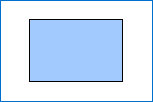
\includegraphics[width=0.2\textwidth]{APS-C_Canon.png}
    \end{figure}

    \columnbreak

    \begin{figure}
        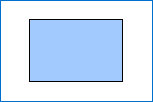
\includegraphics[width=0.2\textwidth]{APS-C_Canon.png}
    \end{figure}
\end{multicols}

\subsection{Crop} \label{subsec:crop}
I sensori più piccoli di un full frame hanno anche un importantissimo fattore di cui è importante tenere conto: il \textbf{crop}.
Crop in inglese significa letterealmente \textit{ritagliare}, ed è quello che in un certo senso succede.

Se sovrapponiamo un full frame e un APS-C vediamo bene come il secondo sensore sia più piccolo del primo. Se usiamo una lente con la stessa identica focale, per riprendere la stessa scena sui due sensori, l'APS-C è in grado di vedere un pezzo più ristretto di scena, come se avessimo zoommato, o, come suggerisce il nome, come se avessimo ritagliato l'inquadratura. Quindi un sensore APS-C \textbf{rispetto} a un full frame appare più zoommato.

\begin{figure}[h]
    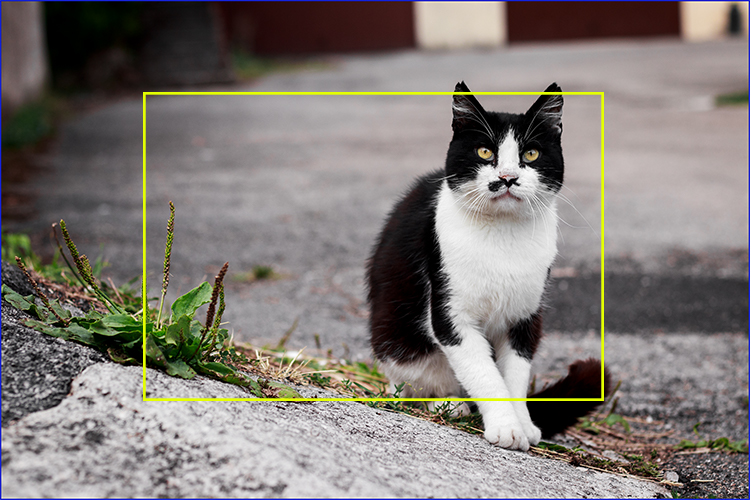
\includegraphics[width=0.6\textwidth]{Gatto_sensori_crop.png}
    \caption{Immaginiamo che l'immagine per intero sia stata ripresa con un full frame; il rettangolo giallo all'interno mostra come la foto sarebbe uscita se fosse stata scattata dalla stessa distanza, con la stessa focale, ma con un sensore APS-C.}
\end{figure}

Quanto croppano i sensori? Dipende da quanto è grande il sensore, più è piccolo e più croppa.

Gli APS-C della Canon croppano con un fattore moltiplicativo di $1.6$; ad esempio, prendiamo un 50mm, su APS-C appare come un 80mm apparirebbe su full frame, perché $50 \cdot 1.6 = 80$.

Gli APS-C della Nikon sono poco più grandi di quelli che usa Canon e croppano con un fattore di $1.5$. Il Micro 4/3 invece croppa $\times 2$.

I fattori di crop sono un informazione ben nota, e non essendoci molti tipi di sensori diversi in commercio (parlando delle dimensioni) non è un'informazione che serve costantemente andare a cercare, ma nel caso volessimo possiamo
facilmente calcolarlo. Basta fare il rapporto tra la lunghezza della diagonale di un full frame e la diagonale del sensore che ci interessa, ovvero applichiamo la seguente formula:
\[ \dfrac{\text{diagonale full frame}}{\text{diagonale sensore di interesse}} \]

Sappiamo quanto sono lunghi i lati di un sensore, e possiamo applicare il \textit{Teorema di Pitagora} per ricavare la diagonale:
\[ d = \sqrt{b^2 + h^2} \]

La diagonale dei sensori full frame è:
\[ d_{full} = \sqrt{36^2 + 24^2} \approx 43.267 \]

La diagonale di un sensore APS-C Canon è:
\[ d_{apsc} = \sqrt{22.2^2 + 14.8^2} \approx 26.681 \]

Quindi il fattore di crop dei sensori APS-C Canon è:
\[ \dfrac{d_{full}}{d_{apsc}} = \dfrac{43.267}{26.681} \approx 1.6 \]


\subsection{Medio formato e oltre} \label{subsec:sensorimedioformato}
Esistono formati più grandi del full frame, vengono detti \textbf{medio formato} e \textbf{grande formato}.

Il \textbf{grande formato} sono tutti i formati dal $4 \times 5$ a salire (in questo caso $4 \times 5$ sono pollici, grossomodo equivalgono a $100mm \times 130mm$).

Alcuni grandi formati sono:
\begin{itemize}
    \item[-] $4 \times 5$
    \item[-] $5 \times 7$
    \item[-] $8 \times 10$
\end{itemize}

\textbf{Medio formato} invece sono tutti i formati più grandi del full frame e più piccoli del $4 \times 5$. Il medio formato è anche detto \textbf{120} o \textbf{220}.

Alcuni medi formati sono:
\begin{itemize}
    \item[-] $6 \times 4.5$
    \item[-] $6 \times 6$
    \item[-] $6 \times 7$
\end{itemize}

All'inizio della fotografia si usavano lastre (e in seguito pellicole) molto grandi, che richiedevano un'attrezzatura e dei costi non banali. Con l'avanzare delle scoperte, delle migliorie delle attrezzature e anche della commercializzazione delle fotografia sono stati creati e si sono diffusi formati più piccoli, come il full frame e l'APS-C.

Questi formati richiedono molto tempo e costi non indifferenti, motivi per i quali sono ancora oggi molto di nicchia, eppure hanno il pregio di fornire immagini di una qualità impareggiabile dai sensori più piccoli.

In commercio oggi si trova qualche macchinetta digitale medio formato, ma solo i corpi macchina costano diverse migliaia di euro, così come tutti gli obiettivi disponibili per medio formato. Per un kit completo si può arrivare sui $20\,000 \euro{}$ e più.

Certamente più accesibile è la fotografia su vecchie fotocamere medio formato analogiche, mentre la fotografia grande formato non si è molto evoluta, si fa ancora su pellicola, e sebbene anche qui i costi siano accessibili ai più, decidere di scattare su grande formato non è solo una scelta stilistica ma quasi un atto di fede.

Notiamo come, essendo formati più grandi del full frame, non hanno un vero e proprio fattore di \textit{crop}, sebbene si usi comunque questo nome. Sui formati più grandi del full frame le focali diminuiscono, diventano più grandangolari.